
\begin{figure}
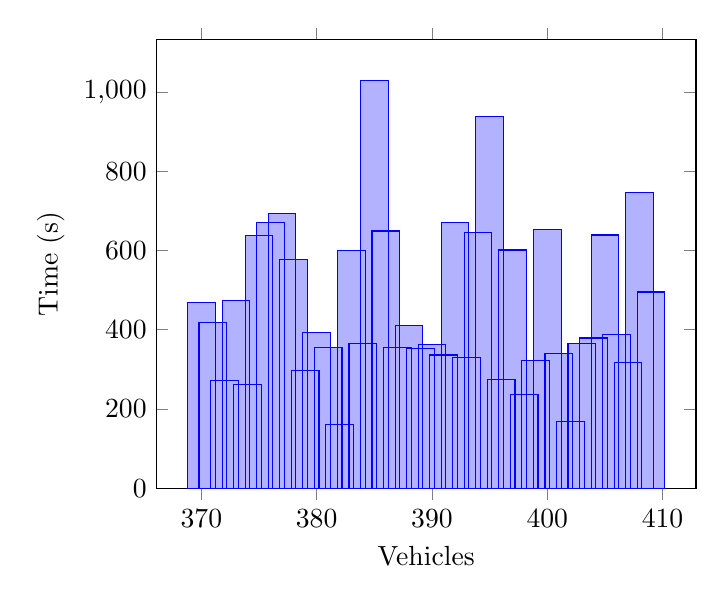
\begin{tikzpicture}
\begin{axis}[
legend style={anchor=west},
xlabel=Vehicles,
ylabel=Time (s),
ymin=0,
ybar,
]
\addplot coordinates {
(394, 645)
(378, 576)
(386, 649)
(395, 939)
(406, 388)
(385, 1029)
(387, 354)
(403, 364)
(375, 638)
(393, 330)
(402, 169)
(389, 353)
(382, 161)
(404, 379)
(381, 354)
(408, 746)
(392, 671)
(400, 653)
(380, 392)
(399, 322)
(373, 474)
(405, 639)
(396, 274)
(391, 336)
(376, 671)
(370, 469)
(383, 600)
(379, 296)
(374, 262)
(397, 601)
(371, 419)
(372, 272)
(377, 694)
(409, 495)
(407, 317)
(398, 236)
(390, 363)
(401, 340)
(388, 411)
(384, 364)
};

\end{axis}
\end{tikzpicture}
\label{tik:time:100:58}
\caption{100 percent diving with GSC on route $58$}
\end{figure}
